%%% Ne pas modifier jusqu'à la ligne 25
\documentclass[a4paper,12pt]{book}
\usepackage[utf8]{inputenc}
\usepackage[french]{babel}
%%\usepackage{CJK}
\usepackage{yhmath}
\usepackage[left=2cm,right=2cm,top=3cm,bottom=2cm, headheight=1.5cm,headsep=1.5cm]{geometry}
\usepackage{amsmath,amsfonts,amssymb,dsfont}
\usepackage{graphicx}
\usepackage{enumitem}		%\enumerate-resume
\usepackage[colorlinks=true,unicode={true},hyperindex=false, linkcolor=blue, urlcolor=blue]{hyperref}
\newcommand{\myref}[1]{\ref{#1} page \pageref{#1}}

\addto\captionsfrench{\def\tablename{Tableau}}  %légendes des tableaux
\renewcommand\thesection{\Roman{section}~-~} 
\renewcommand\thesubsection{\Roman{section}.\Alph{subsection}~-~} 
\renewcommand\thesubsubsection{\Roman{section}.\Alph{subsection}.\arabic{subsubsection}~-~} 

\newcommand{\conclusion}[1]{\newline \centerline{\fbox{#1}}}

\setcounter{secnumdepth}{3}
\parindent=0pt

\usepackage{fancyhdr}
\pagestyle{fancy}

\lhead{SJTU-ParisTech} 
%%%%%%%%%%%%%%%%%%%%%%%%%%%%%%%%%%
\chead{DM1}
\rhead{Daniel 518261910024}

\begin{document}
\renewcommand{\labelitemi}{$\blacktriangleright$}
\renewcommand{\labelitemii}{$\bullet$}


\section{énergie libre d’un gaz parfait}
\subsection{U(T)}
Par les relations de Gibbs-Helmholtz, on a $-\frac{U}{T^2}=\left(\frac{\partial (F/T)}
{\partial T}\right)_V$, donc:
\begin{align*}
U&=-T^2\left(\frac{\partial (F/T)}{\partial T}\right)_V\\
 &=-T^2\left(\frac{\partial}{\partial T}\frac{3}{2}nR\left(1-\frac{T_0}{T}-\ln\frac{T_0}{T}
 -\frac{2}{3}\ln\frac{V_0}{V}\right)+\frac{U_0}{T}-S_0\right)_V\\
 &=-T^2\left(\frac{3}{2}nR\left(\frac{T_0}{T^2}-\frac{1}{T}\right)\right)-\frac{U_0}{T^2}(-T^2)\\
 &=-\frac{3}{2}nRT_0+\frac{3}{2}nRT+U_0\\
 &=\frac{3}{2}nR(T-T_0)+U_0\\
\end{align*}
On a donc $\boxed{U(T)=\frac{3}{2}nR(T-T_0)+U_0}$, ce qui est correspondant à $dU=C_v\,dT$, où $C_v=
\frac{3}{2}nR$ pour un gaz parfait monoatomique.

\subsection{S(T,V)}
Par les relations différentielles, on a $S=-\left(\frac{\partial F}{\partial T}\right)_V$, donc:
\begin{align*}
S&=-\frac{3}{2}nR\left(1-\left(1+\ln\frac{T}{T_0}\right)+\frac{2}{3}\ln\frac{V}{V_0}\right)+S_0\\
 &=\frac{3}{2}nR\ln\frac{T}{T_0}+nR\ln\frac{V}{V_0}+S_0\\
\end{align*}
On a donc $\boxed{S(T,V)=\frac{3}{2}nR\ln\frac{T}{T_0}+nR\ln\frac{V}{V_0}+S_0}$, ce qui est 
correspondant à $dS=nR\ln\frac{V_f}{V_i}+C_v\ln\frac{T_f}{T_i}$, où $C_v=
\frac{3}{2}nR$ pour un gaz parfait monoatomique.

\section{potentiel thermodynamique}
On divise l'évolution en trois étapes. C'est une transformation monotherme, monobare (contact avec l'atomsphère). 
On suppose que le système considéré est fermé. 
\begin{figure}[h]
    \begin{center}
    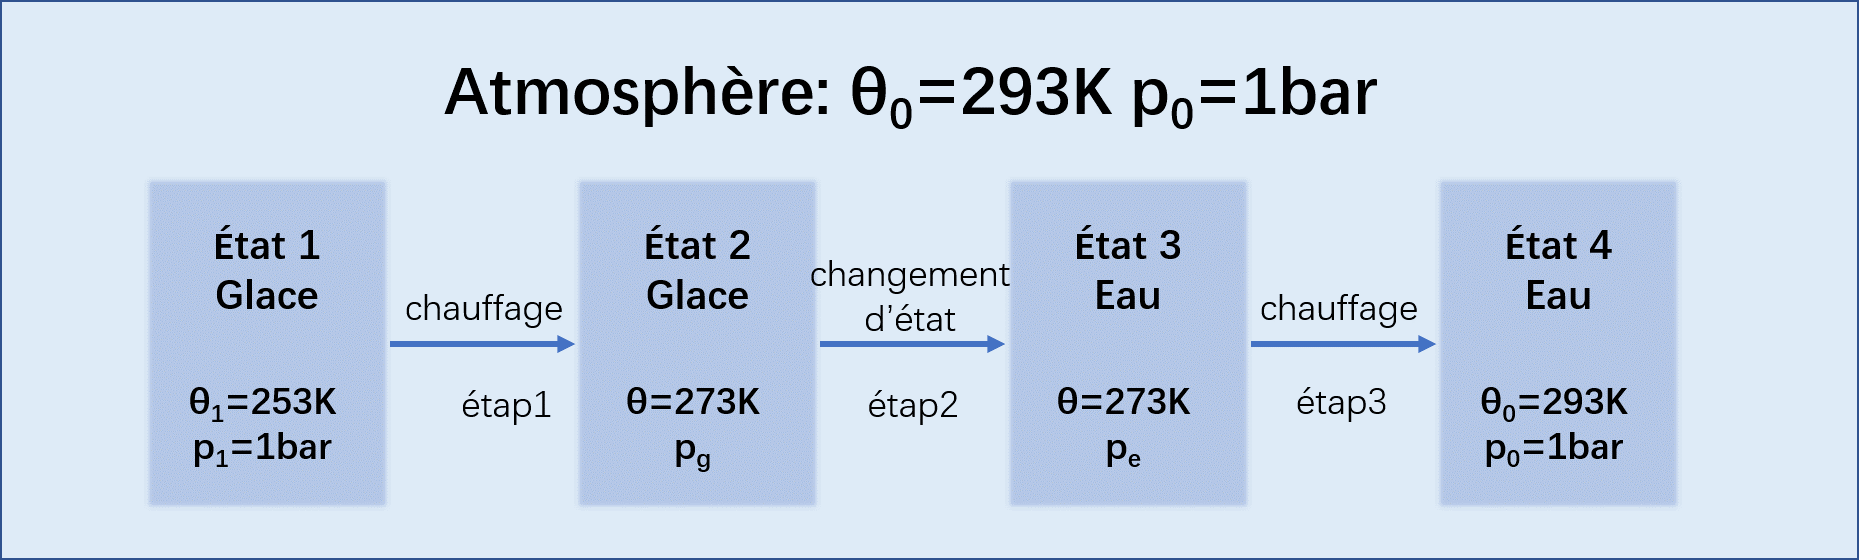
\includegraphics[scale=0.5]{dm1.png}
    \end{center}
    \caption{Division des étapes}
\end{figure}
\subsection{chauffage de la glace}
La glace considérée comme phase condensée: $C_v=C_P=C_{glace}$, 
$dS=C_{glace}\frac{d\theta}{\theta}$, $dH=dU$. Donc
\begin{align*}
    dG_{etap1}^*&=dU-\theta_0\,dS\\
                       &=dU-\theta_0(\delta S_{cr}+\frac{\delta Q}{\theta_g})\\
                       &=dU-\frac{\theta_0}{\theta_g}\,dU-\theta_0\delta S_{cr}\\
                       &=\left(1-\frac{\theta_0}{\theta_g}\right)C_{glace}\,d\theta_g-\theta_0\delta S_{cr}\\
\end{align*}
où $\theta_g\in[253K,273K]$ la température de chaque instant, qui est inférieur à $\theta_0=293K$
et on a $dU=\delta Q$ selon le première loi de thermodynamiques.
A.N. on a $\boxed{dG^*_{etap1}<0}$ lorsque $\theta_0>\theta_g, \delta S_{cr}\geq 0$, 
Ce qui montre que cette étape est spontanée.

\subsection{étap de fusion}
On a $dG_{fus}=dH_{fus}-\theta_0dS_{fus}$, avec $dS_{fus}=\frac{dH_{fus}}{\theta_{fus}}$ pour unchangement d'état, où $\theta_{fus}=273K$ 
donc $dG_{fus}= (1-\frac{\theta_0}{\theta{fus}})dH_{fus}$. A.N. $\boxed{dG_{fus}=-0.07dH_{fus}<0}$ car $dH_{fus}>0$, l'évolution est spontanée.

\subsection{chauffage de l'eau}
Par la même méthode, on a 
\begin{align*}
    dG^{*}_{etap2}&=dU-\theta_0\,dS\\
                           &=dU-\theta_0(\delta S^{'}_{cr}+\frac{\delta Q^{'}}{\theta_e})\\
                           &=\left(1-\frac{\theta_0}{\theta_e}\right)C_{eau}\,d\theta_e-\theta_e\ delta S^{'}_{cr}\\
\end{align*}
où $\theta_e\in[273K,293K]$ la température de chaque instant, qui est inférieur à $\theta_0=293K$.

A.N. on a $\boxed{dG^{*}_{etap2}<0}$, lorsque $\theta_0>\theta_e, \delta S_{cr}^{'} \geq 0$, 
Ce qui montre que cette étape est spontanée.


Finalement, d'après  le potentiel thermodynamique, on peut déduire le sens d’évolution de ce système
couplé avec le milieu extérieur
\end{document}